\documentclass[a4paper]{article}
\usepackage[french]{babel}
\usepackage[utf8]{inputenc}
\usepackage[T1]{fontenc}
\usepackage{graphicx}   % pour les images
\usepackage{hyperref}   % pour les références
\usepackage{amssymb}    % pour les symboles de maths comme \mathbb{R}
\usepackage{mathtools}  % pour rajouter \text dans un environment math
\usepackage{subcaption} % pour les subfigures
\usepackage{float}      % truc pour mettre les images à la bonne place
\usepackage[style=ieee]{biblatex}
\addbibresource{ref.bib}
\bibliography{ref.bib}

\hypersetup{
    colorlinks=true,
    linkcolor=blue,   % Couleur des liens internes (table des matières, références)
    citecolor=green,  % Couleur des liens vers les références bibliographiques
    filecolor=magenta,% Couleur des liens vers les fichiers
    urlcolor=blue     % Couleur des liens vers les URL
}


\title{Rapport PSTALN}
\author{Cléa Han, Yanis Labeyrie et Adrien Zabban}
\date{janvier 2024}

\begin{document}

\maketitle
\bigskip
\tableofcontents
\newpage

\section{Introduction}

Le but de ce projet est de faire un modèle de langage capable de prédire les morphologies des mots d'une phrase
(\textit{morphy}), comme le montre la Figure~\ref{fig: example morphy}. L'ensemble des \textit{morphy} 
est recensé dans les Annexes (section~\ref{sec: Annexes}, Figure~\ref{fig: all morphy}).

\begin{figure}[H]
    \centering
    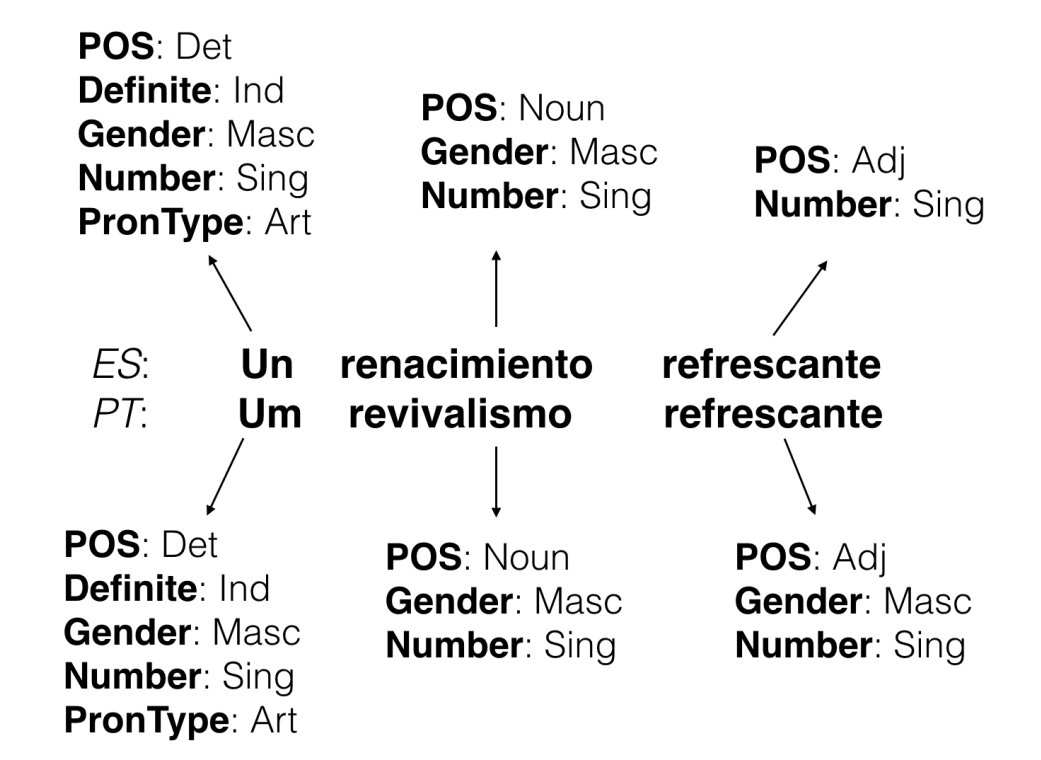
\includegraphics[width=0.5\textwidth]{morphy.png}
    \caption{Tag morphologique d'une phrase portugaise et sa traduction en espagnol.
    Image tirée de~\cite{malaviya-etal-2018-neural}}
    \label{fig: example morphy}
\end{figure}    

Nous allons aussi nous demander si le fait d'ajouter un prétraitement de la phrase va améliorer
les performances. L'idée de ce prétraitement est de faire prédire le balisage de séquence
prototypique (\textit{pos}) des mots, comme le montre la Figure~\ref{fig: example pos}. L'ensemble des \textit{pos} 
est recensé dans les Annexes (section~\ref{sec: Annexes}, Figure~\ref{fig: all pos}).

\begin{figure}[H]
    \centering
    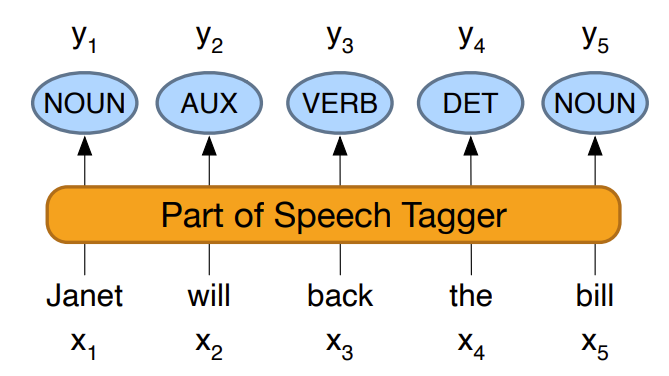
\includegraphics[width=0.5\textwidth]{pos.png}
    \caption{La tâche d'étiquetage des parties du discours : la mise en correspondance des mots d'entrée 
    $x_1, x_2,..., x_n$ avec les étiquettes \textit{pos} de sortie $y_1, y_2,..., y_n$.
    Image tirée de~\cite{pos}}
    \label{fig: example pos}
\end{figure} 

\section{Données}

Nous avons utilisé le dataset Universal Dependencies 2.13 ~\cite{11234/1-5287}, qui comporte 146 langues dont l'anglais
et le français. Dans ce projet, nous nous sommes seulement concentrés sur le français.
Le dataset en français contient un ensemble de 47498 phrases, avec 849476 mots, et 76048 mots uniques.
Ce dataset possède des phrases, la liste de mots composant ses phrases, les \textit{pos} et \textit{morphy} qui sont associés à chacun de ses mots. Au total, nous avons recensé $19$ \textit{pos} et 
$28$ \textit{morphy} différents.

\subsection{Padding}

Les phrases données au modèle doivent être toutes exactement de la même longueur pendant l'entraînement. 
Notons $K$ la longueur des séquences\footnote{Nous appelons séquence, les suites de mots de même taille.}. Nous créons donc des 
tokens <PAD> pour équilibrer les longueurs des phrases.
Nous avons choisi d'utiliser une méthode naïve pour créer nos séquences qui consiste à couper chaque phrase pour former les séquences
de $K$ mots, et de rajouter si besoin des tokens <PAD> pour terminer la dernière séquence. Nous avons choisi de prendre $K=10$.

\subsection{Gestion des mots inconnus}

Nous avons, avant l'entraînement du modèle, appris un vocabulaire de mots qui fait la correspondance entre les mots et un nombre unique.
Le vocabulaire a été fait seulement sur les mots qui sont dans la base de données d'entraînement. C'est donc pour cela qu'il peut
arriver que des mots de la base de données de validation ou de test ne soient pas reconnus par le vocabulaire et donc par le modèle.
Pour gérer ces mots inconnus, nous avons décidé de leur attribuer le token particulier : <UNK>. Pour que le modèle
apprenne l'embedding de ce mot, il faut alors rajouter artificiellement des mots inconnus dans le corpus d'entraînement. Nous avons
donc remplacé chaque mot de ce corpus par <UNK> avec une probabilité de $1\%$.


\subsection{Encodage des labels}

Pour encoder les \textit{pos}, nous avons seulement créé une liste de tous les \textit{pos} et avons encodé les \textit{pos} avec 
leurs indices dans la liste.
Nous avons aussi ajouté le \textit{pos} <PAD> pour que le token de padding soit catégorisé dans ce \textit{pos}.


Pour les \textit{morphy}, cela a été plus compliqué, car un mot peut avoir plusieurs \textit{morphy} associés, avec des valeurs
différentes. Nous avons décidé d'encoder une suite de \textit{morphy} par une liste de nombre de longueurs $28$ et les éléments
sont les indices des possibilités de chaque
\textit{morphy}. Par exemple : le label \textit{Emph=No|Number=Sing|Person=1|PronType=Prs} est encodé par la liste ci-dessous :

[0, 0, 1, 0, 1, 2, 9, 0, 0, 0, 0, 0, 0, 0, 0, 0, 0, 0, 0, 0, 0, 0, 0, 0, 0, 0, 0, 0]

Comme pour le \textit{pos}, nous avons aussi ajouté un \textit{morphy} pour le padding. Étant donné que le \textit{morphy} qui possède
le plus de possibilités en possède 13, quand nous encodons les labels en one-hot, nous avons un tensor de shape
$(19)$ pour les \textit{pos} et un tensor de shape $(28, 13)$ pour les \textit{morphy}.


\section{Modèle}

\subsection{Architecture des \textit{pos}}

Le modèle, que nous appelons \textit{GET\_POS}, est constitué d'une couche d'embedding pour apprendre les plongements
des mots. Les données passent alors dans une couche LSTM bidirectionnel, puis dans une couche dense (fully connected layers),
avec une sortie à 19 éléments représentant les probabilité de chaque classe \textit{pos}. Nous avons utilisé du 
dropout sur les neurones des couches LSTM et dense, avec un taux d'oublie de $1\%$. Entre ces 3 couches, nous avons 
aussi ajouté la fonction d'activation ReLU~\cite{DBLP:journals/corr/abs-1803-08375}. Nous avons utilisé la CrossentropyLoss 
comme fonction de coût, l'optimizer Adam~\cite{kingma2014adam}. Ce modèle est représenté sur la Figure~\ref{fig: model getpos}.
Nous avons donc en entrée une matrice de taille $B \times K$, contenant l'indice des mots, où $B$ est la taille du batch.
 Et le modèle retourne un tensor de taille $B \times K \times 19$, contenant les probabilités des \textit{pos} pour chaque mot.

\begin{figure}[H]
    \centering
    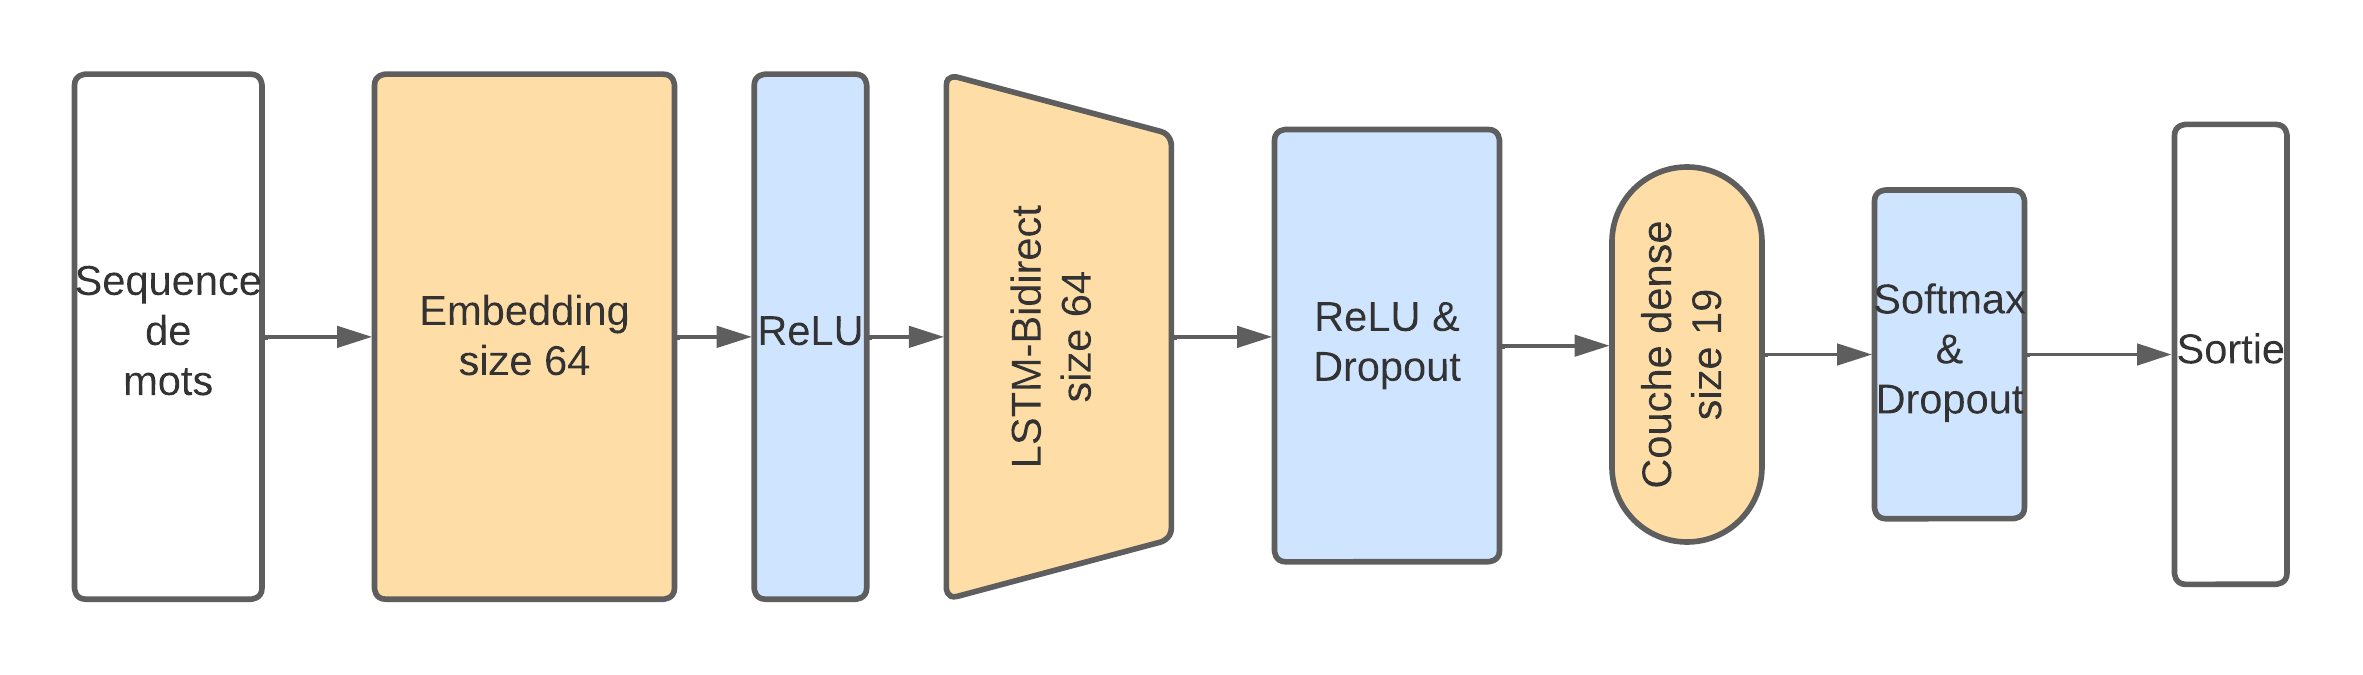
\includegraphics[width=0.6\textwidth]{get_pos.png}
    \caption{Modèle \textit{GET\_POS}}
    \label{fig: model getpos}
\end{figure} 

\subsection{Architecture des \textit{morphy}}

Pour la tâche de prédiction des traits morphologiques, la difficulté est supérieure. En effet, pour cette tâche 
il faut prédire pour chaque mot de la phrase à la fois son rôle dans la phrase (Verbe, Nom, etc.) mais aussi, 
pour chacune de ses classes, prédire des attributs (singulier, pluriel, etc.). Nous avons donc créé plusieurs 
architectures différentes que nous allons présenter. Nous avons aussi dû modifier la fonction de coût par 
la moyenne des crossentropy sur les 28 \textit{morphy} différents. Nous avons utilisé l'optimizer Adam~\cite{kingma2014adam},
et avons ajouté un gradient decay, qui fait que le learning rate est divisé par deux lors des epochs 10 et 20.

\subsubsection{Modèle \textit{SUPERTAG}}

Le modèle commence par une couche d'embedding pour deux couches de LSTM bidirectionnel. Ensuite, on fait passer les données 
dans 3 couches denses cachées dont la dernière contient $364$ neurones
\footnote{Nous avons pris $364$ neurones car $364 = 28 \times 13$.}
Avant que nos données sortent du modèle, elles ont une
taille de $B \times K \times 364$. On \textit{reshape} alors les données pour avoir une sortie de taille 
$B \times K \times 28 \times 13$. La Figure~\ref{fig: model supertag} représente ce modèle.

\begin{figure}[H]
    \centering
    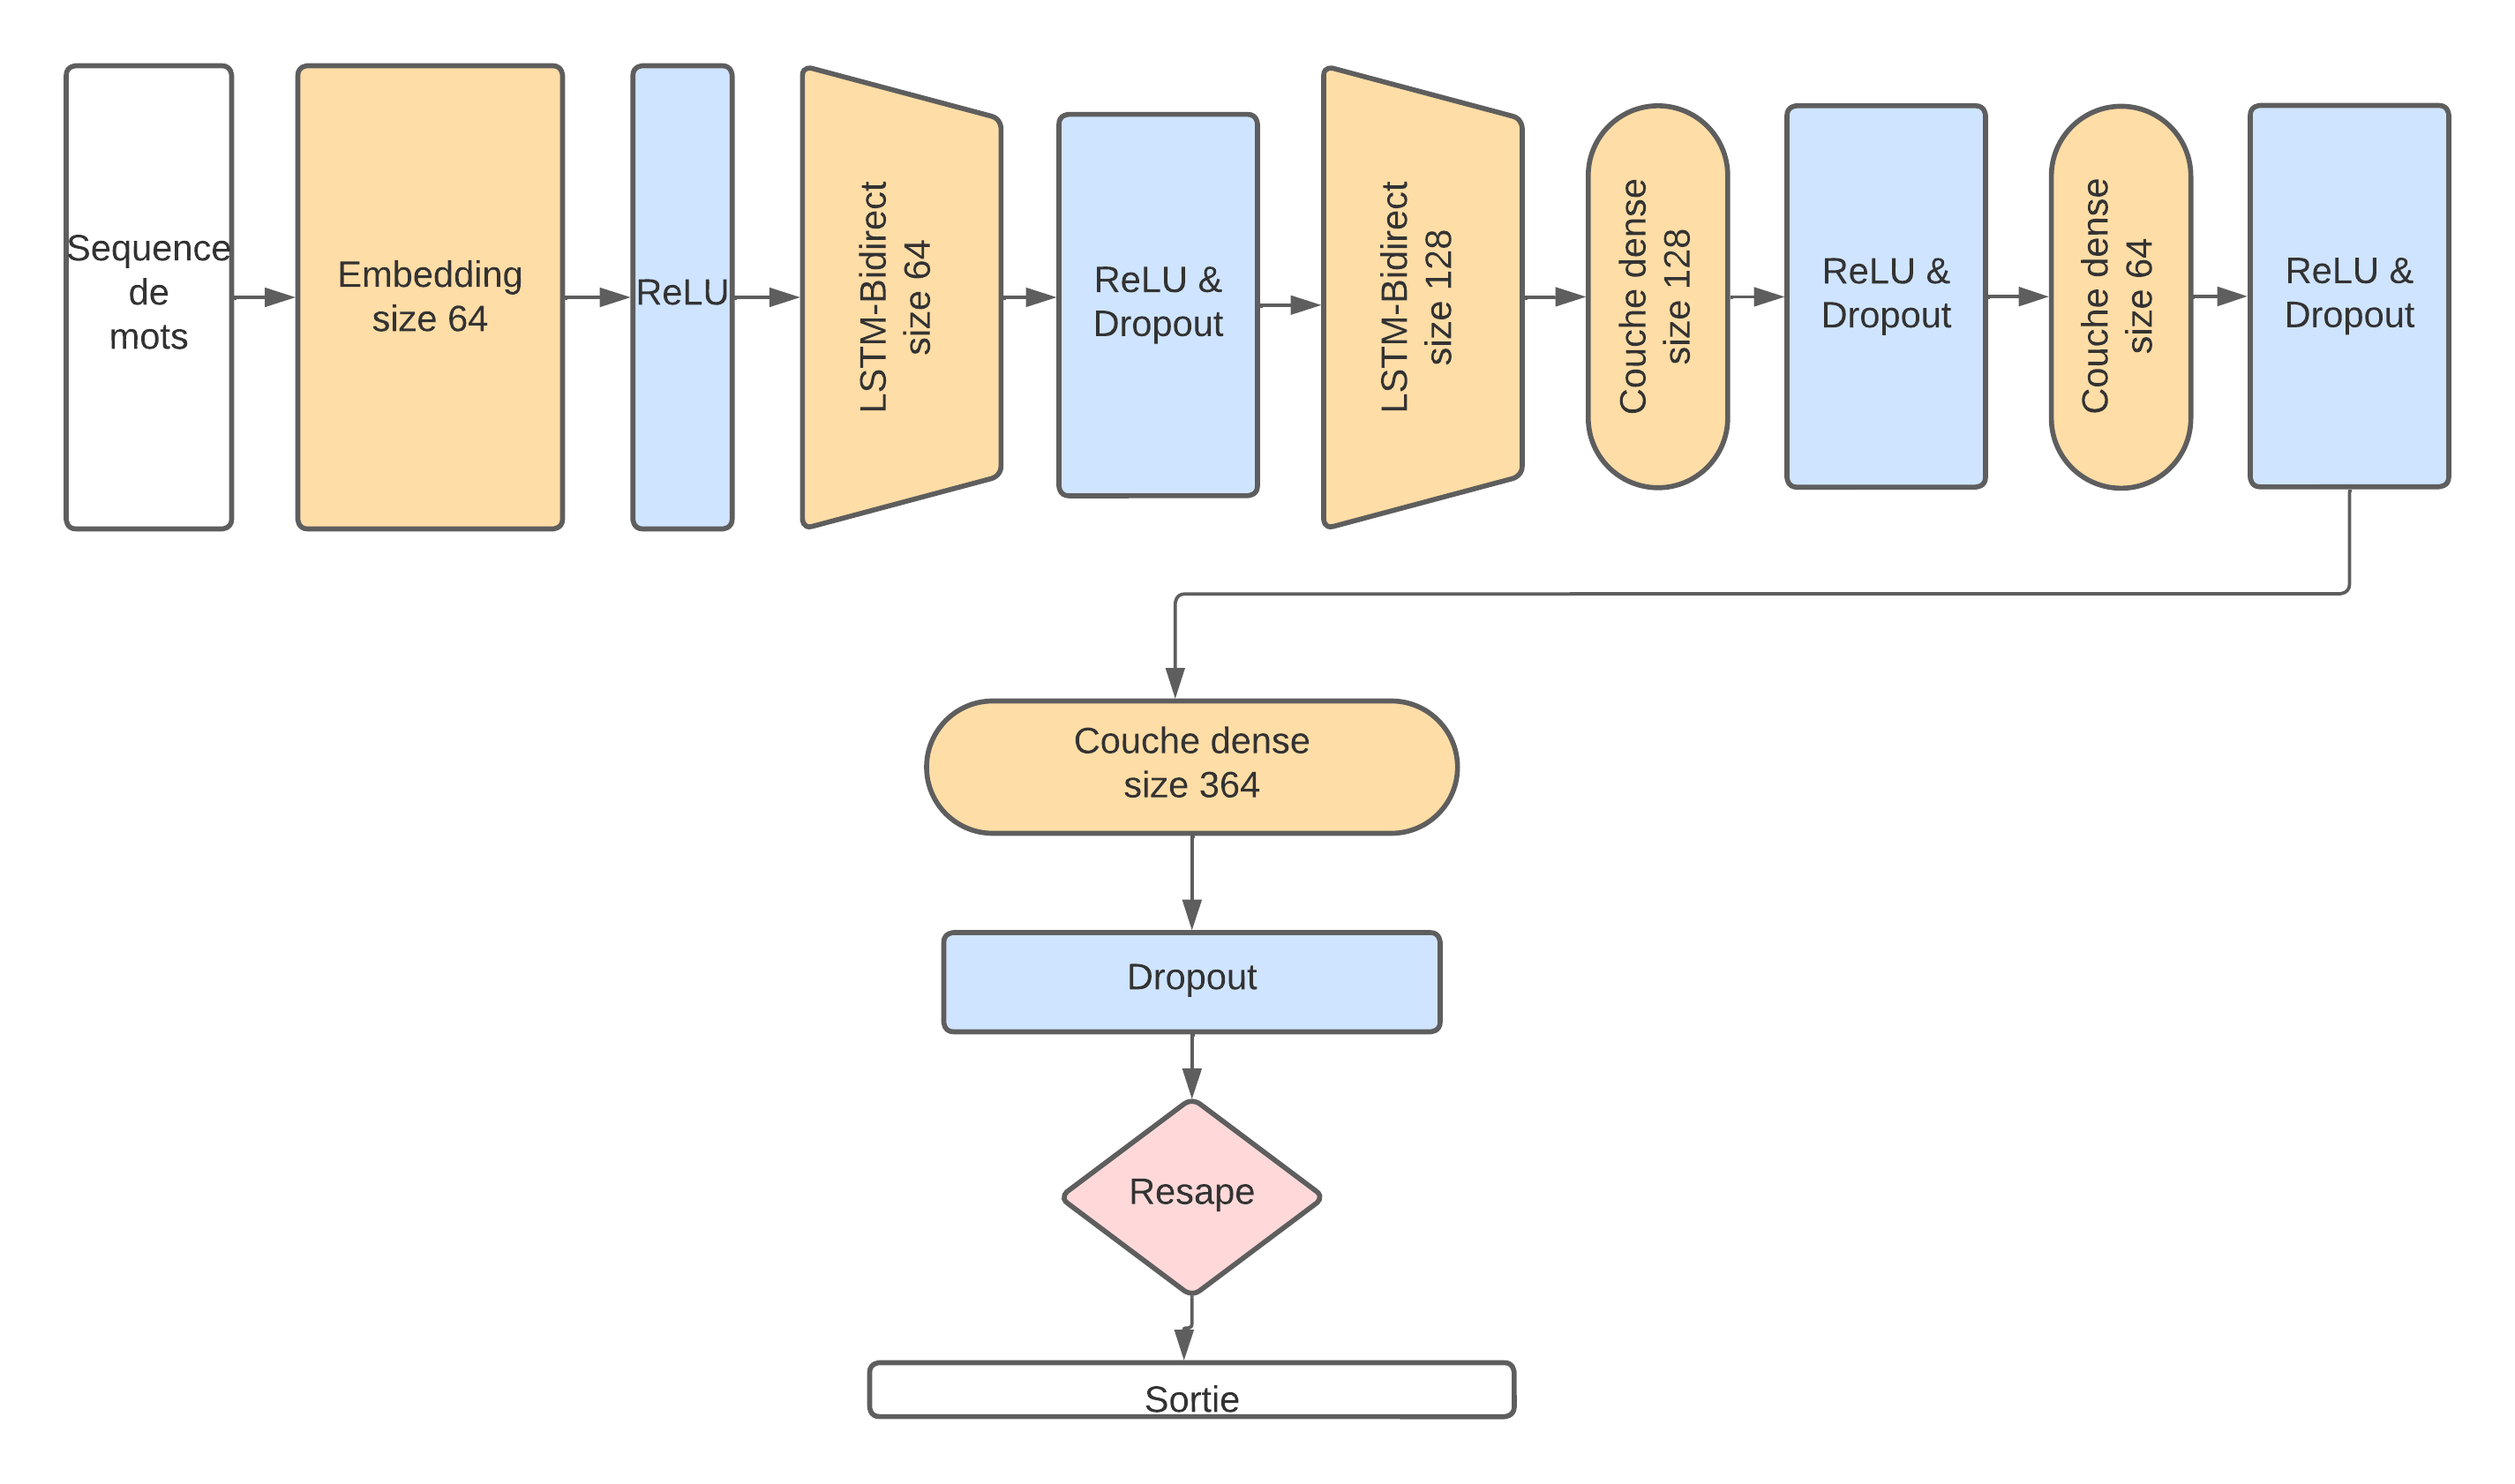
\includegraphics[width=0.7\textwidth]{get_morphy_supertag.png}
    \caption{Modèle \textit{SUPERTAG}}
    \label{fig: model supertag}
\end{figure}

\subsubsection{Modèle \textit{SEPARATE}}

On reprend le même début que le modèle \textit{SUPERTAG} et l'on change la dernière couche. Au lieu de prédire tous les 
\textit{morphy} en même temps avec une seule couche dense, on va avoir 28 couches denses (une par \textit{morphy}). Chaque couche
va alors prédire les probabilités liées à son \textit{morphy}. On va alors ajouter, à chaque prédiction des couches, des $- 1000$
pour obtenir un vecteur de taille $13$ pour tous les mots
\footnote{On a voulu mettre des $-\infty$ car cela permettait d'avoir une probabilité de $0$ après le softmax. Cependant, 
lorsque l'on faisait cela, on avait une loss avec une valeur de \textit{not a number}, donc on a décidé de mettre $-1000$ à 
la place.}.
On va ensuite concaténer tous les résultats avec une sortie de 
taille $B \times K \times 28 \times 13$. La Figure~\ref{fig: model separate} représente ce modèle.

\begin{figure}[H]
    \centering
    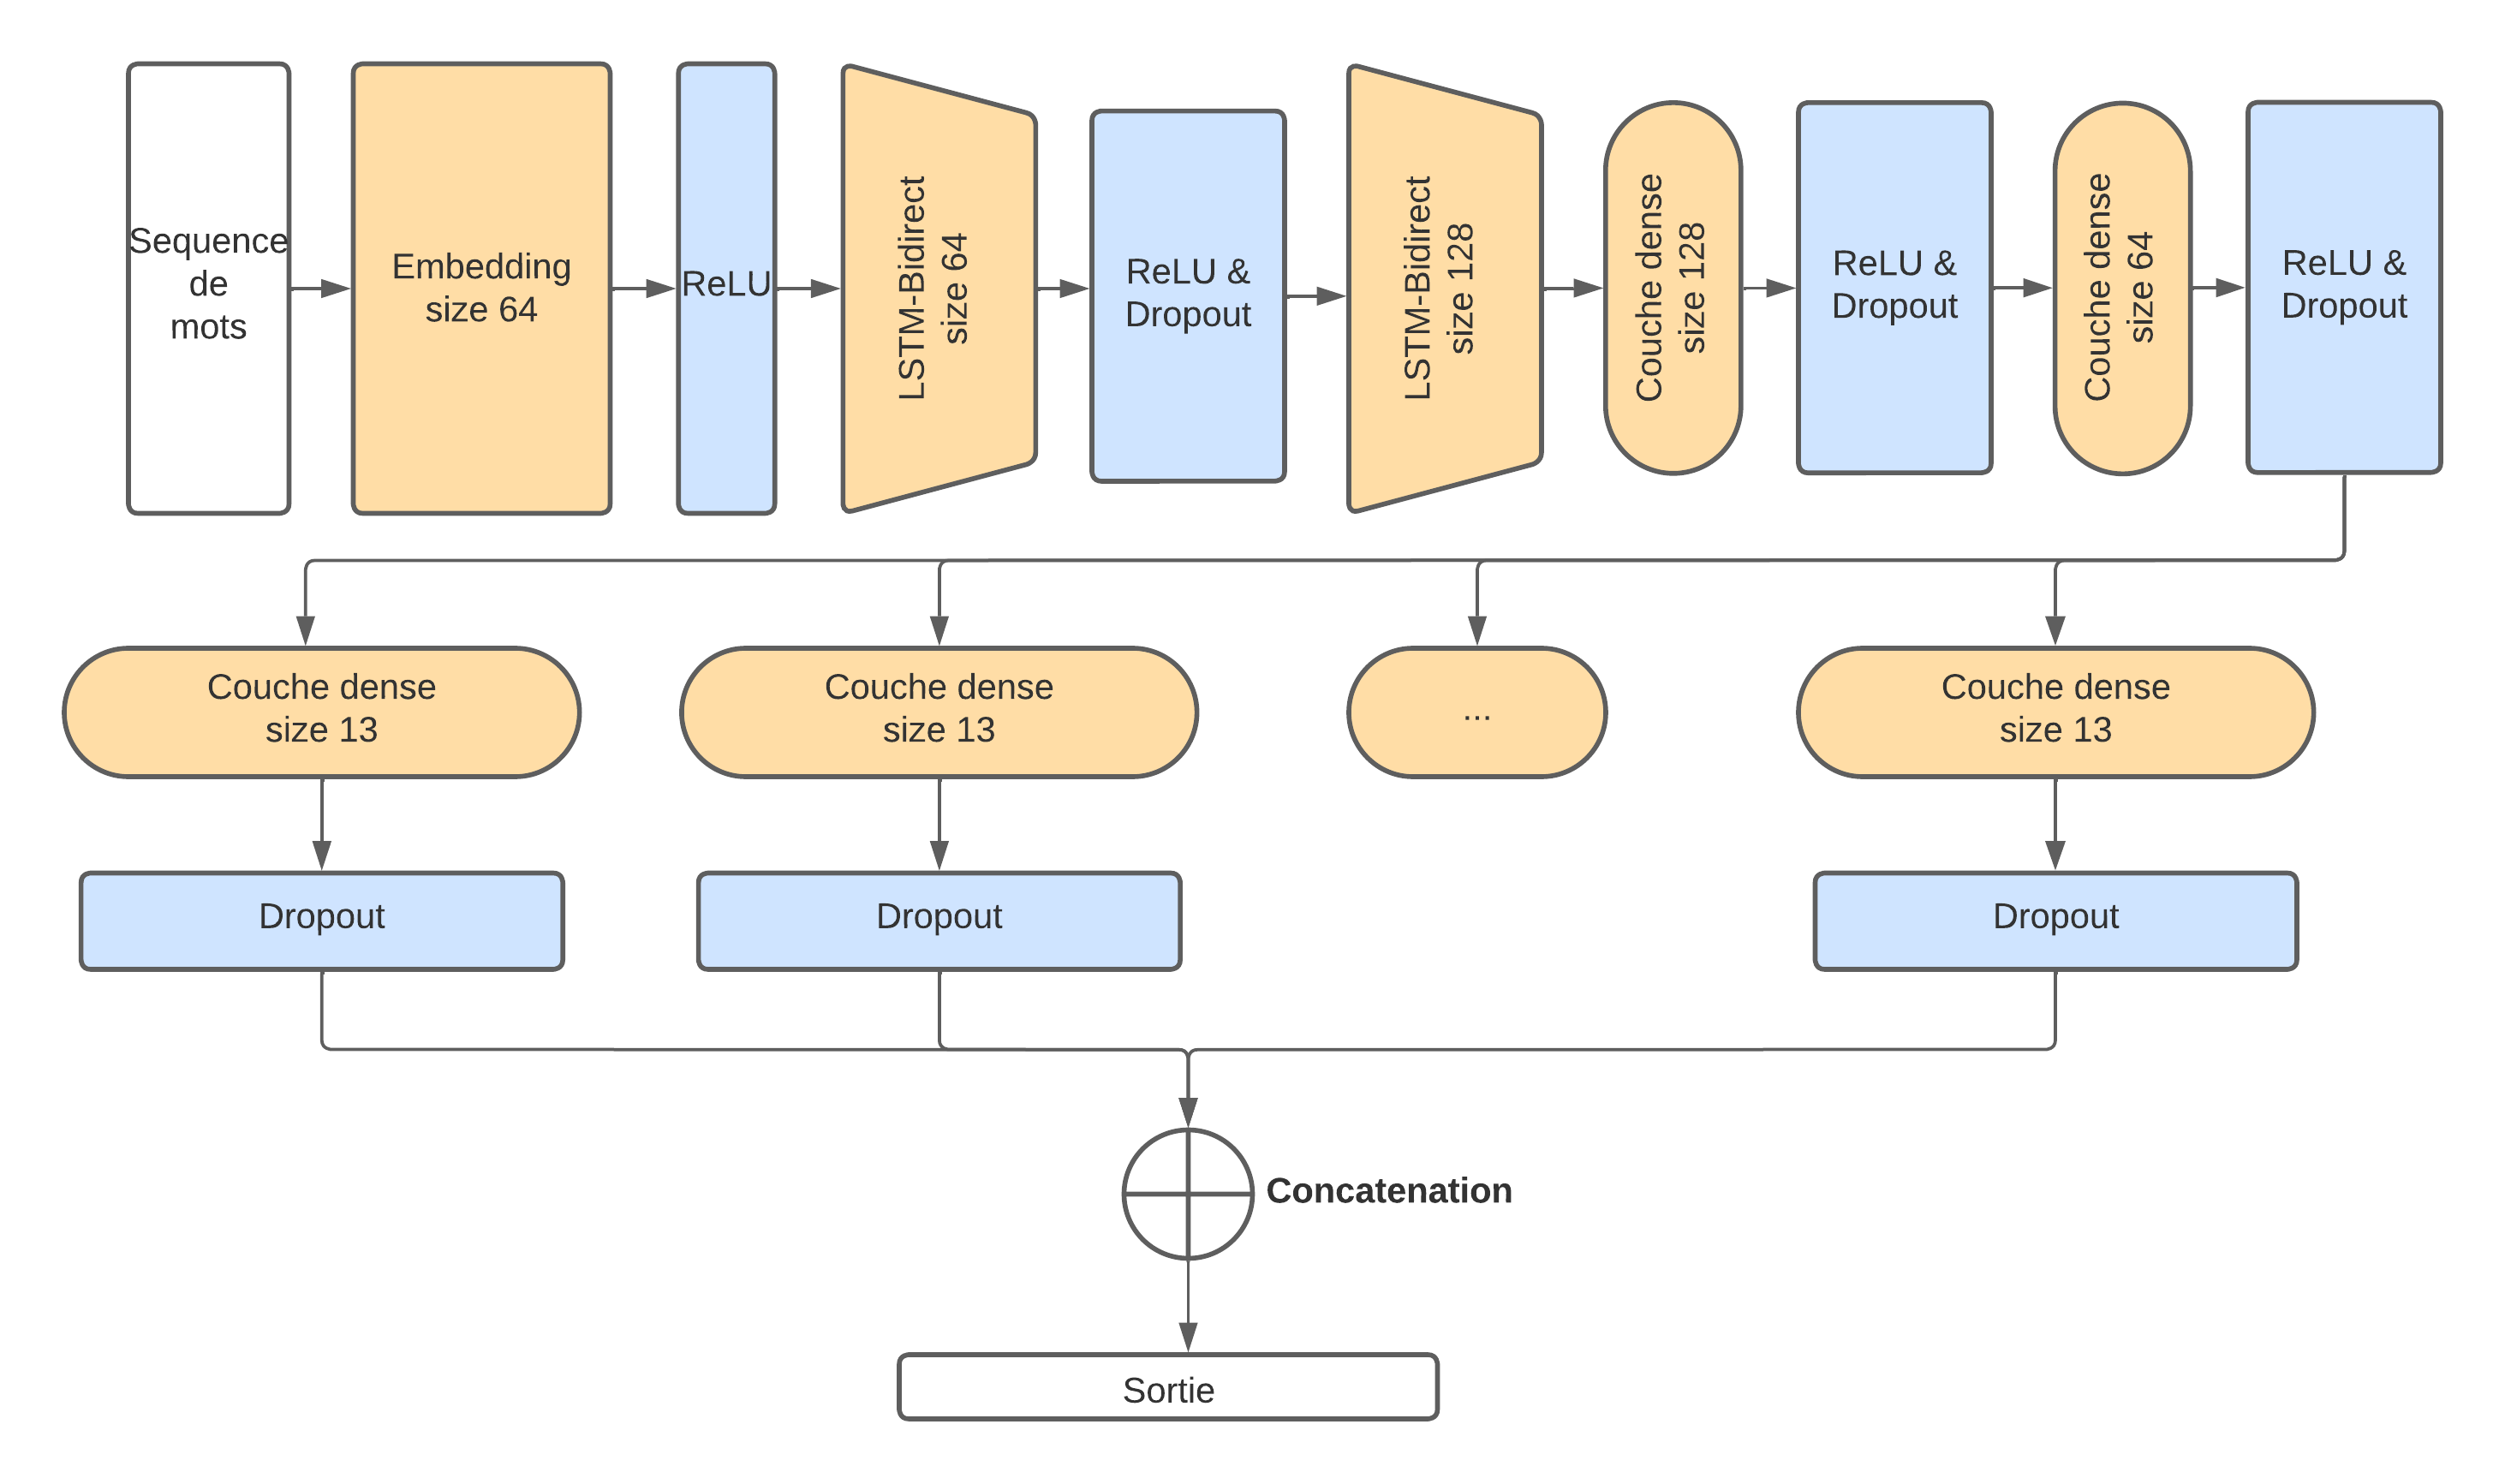
\includegraphics[width=0.7\textwidth]{get_morphy_separate.png}
    \caption{Modèle \textit{SEPARATE}.}
    \label{fig: model separate}
\end{figure}

\subsubsection{Modèle \textit{FUSION}}

L'idée de ce modèle est d'utiliser la prédiction du modèle \textit{GET\_POS} pour aider le modèle \textit{SEPARATE}.
On fait passer les données dans les 2 couches de LSTM, et en sortie, on va concaténer la sortie du LSTM avec la sortie
d'un modèle \textit{GET\_POS} pré-entraîné.
La Figure~\ref{fig: model fusion} représente ce modèle.

\begin{figure}[H]
    \centering
    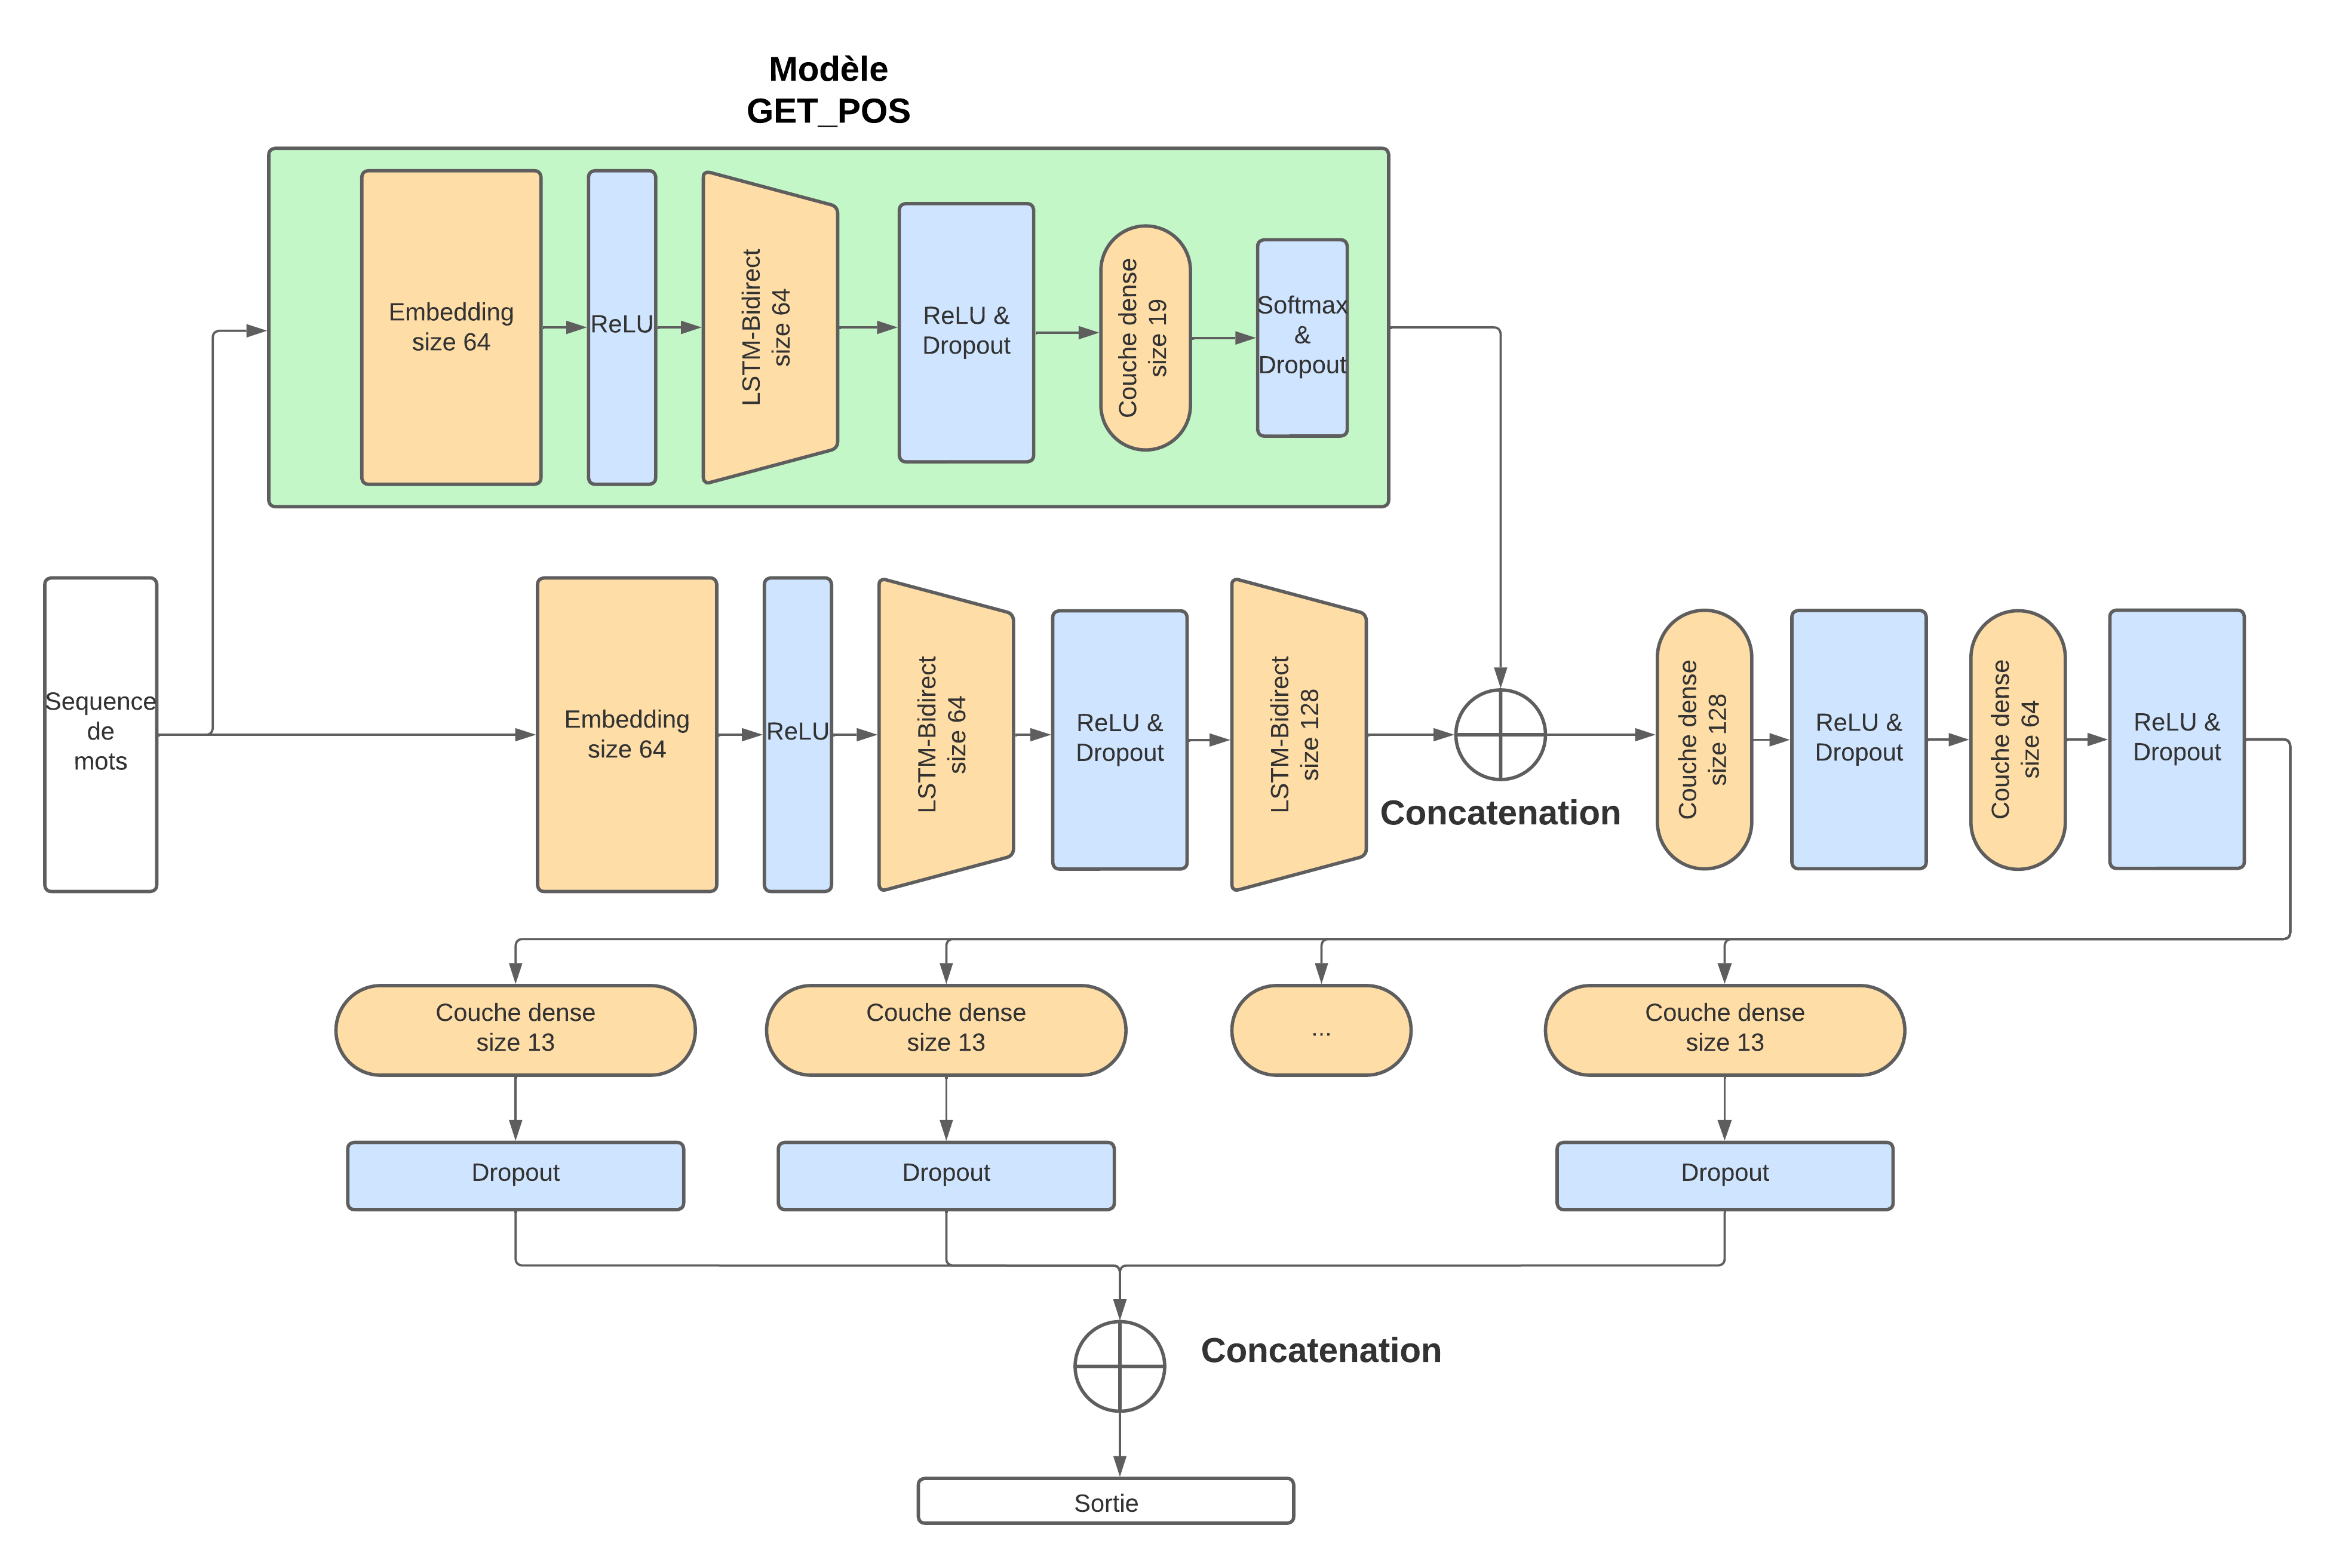
\includegraphics[width=0.7\textwidth]{get_morphy_fusion.png}
    \caption{Modèle \textit{FUSION}}
    \label{fig: model fusion}
\end{figure}


\section{Mesurer les performances des modèles}

\subsection{Mes métriques}

Pour pouvoir mesurer les performances de ces modèles, nous avons mis en place plusieurs métriques. Pour la prédiction de 
\textit{pos}, nous avons utilisé l'accuracy micro et macro. La première nous donne l'accuracy de la prédiction et la deuxième
nous donne la moyenne de l'accuracy sur chacune des classes. 

Pour la prédiction de \textit{morphy}, nous avons aussi utilisé l'accuracy micro, et nous avons aussi implémenté une 
métrique qu'on a appelée \textit{all good}, qui fait la moyenne des mots dont la prédiction de tous les \textit{morphy}
sont justes. Si la métrique vaut $0.2$, cela veut dire qu'il y a 1 mot sur 5 dont la prédiction est totalement bonne.

\subsection{La baseline}

Nous avons implémenté une \textit{BASELINE}, qui prédit les \textit{morphy}, afin d'effectuer des comparaisons de performances avec nos modèles.
Cette baseline s'appuie sur un modèle simple où un dictionnaire est créé et parcourt l'ensemble des données d'entraînements afin de 
récolter tous les mots qu'il n'a jamais croisés et leur label. Ainsi, le dictionnaire indique le vocabulaire du texte en lui assignant
le premier label croisé lors du parcours du dataset d'entraînement.

\section{Résultats}

\subsection{Résultats pour la prédiction de \textit{pos}}
Nous avons donc lancé un entraînement de notre réseau \textit{GET\_POS} sur 20 epochs et 
nous avons obtenu une accuracy de validation d'environ $95\%$ ce qui dénote que le réseau a réussi à apprendre 
correctement cette tâche d'étiquetage, comme le montre la Figure~\ref{fig: train getpos} :

\begin{figure}[H]
    \centering
    \begin{subfigure}{0.32\textwidth}
        \centering
        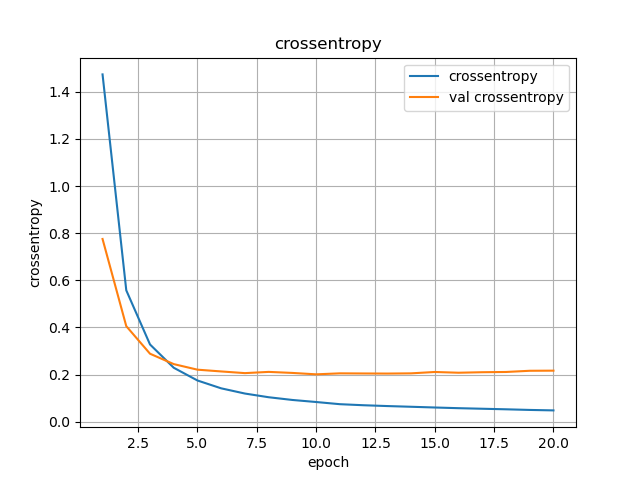
\includegraphics[width=\linewidth]{../logs/get_pos/crossentropy.png}
    \end{subfigure}
    \begin{subfigure}{0.32\textwidth}
        \centering
        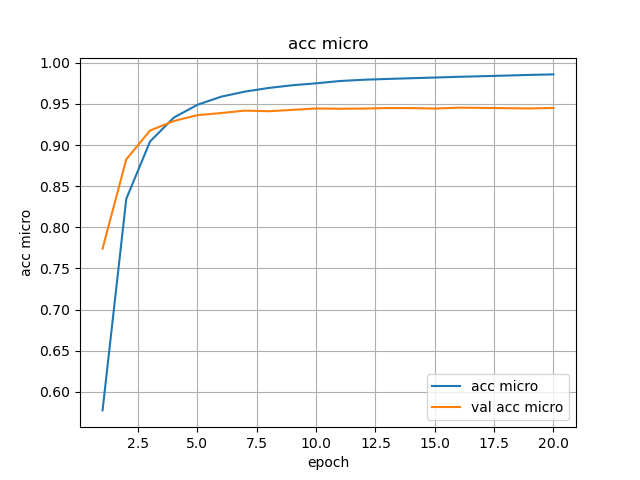
\includegraphics[width=\linewidth]{../logs/get_pos/acc micro.png}
    \end{subfigure}
    \begin{subfigure}{0.32\textwidth}
        \centering
        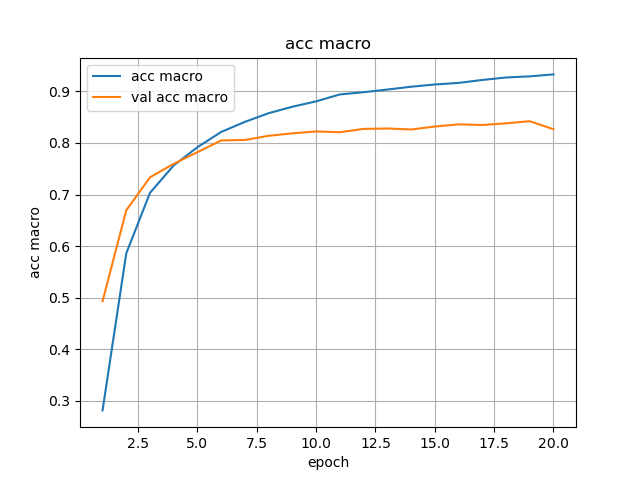
\includegraphics[width=\linewidth]{../logs/get_pos/acc macro.png}
    \end{subfigure}
    \caption{Valeurs de la loss et des métriques d'entraînement et de validation en fonction des epochs.}
    \label{fig: train getpos}
\end{figure}

Nous avons un apprentissage satisfaisant du modèle comme en témoignent les Figures~\ref{fig: train getpos}. 
L'accuracy micro est relativement meilleure en termes de performances et de stabilité que l'accuracy macro.

On constate que la valeur de l'accuracy de validation est un peu plus faible que celle d'entraînement, cela 
s'explique par plusieurs facteurs, notamment la difficulté du modèle à généraliser aux nouveaux mots inconnus.


\begin{table}[H]
    \centering
    \begin{tabular}{|c|c|c|c|}
        \hline
        Nom du modèle & crossentropy & accuracy micro & accuracy macro \\
        \hline
        \textit{GET\_POS} & 0.204 & 0.944 & 0.816\\
        \hline
    \end{tabular}
    \caption{Résultats du modèle \textit{GET\_POS} sur la base de données de teste.}
    \label{tab:test getpos}
\end{table}

Les résultats du Table~\ref{tab:test getpos} témoignent d'une performance satisfaisante du modèle POS avec une accuracy micro 
de $94,4\%$. Néanmoins, si on souhaite d'intéresser à l'accuracy micro, nous atteignons une accuracy de $81,6\%$.

\subsection{Résultats la prédiction des \textit{morphy}}

\begin{figure}[H]
    \centering
    \begin{subfigure}{0.32\textwidth}
        \centering
        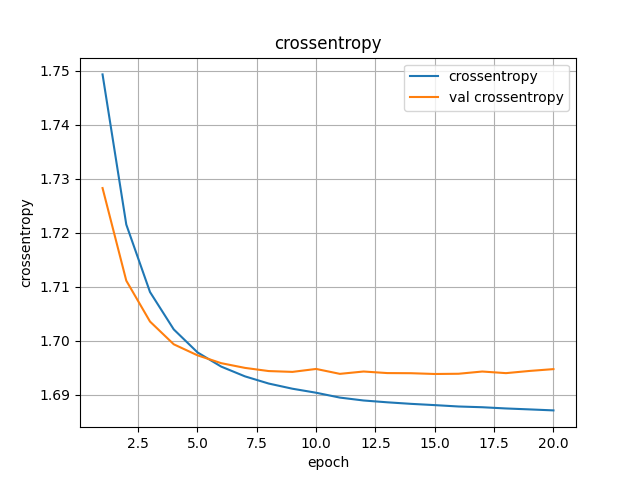
\includegraphics[width=\linewidth]{../logs/supertag/crossentropy.png}
    \end{subfigure}
    \begin{subfigure}{0.32\textwidth}
        \centering
        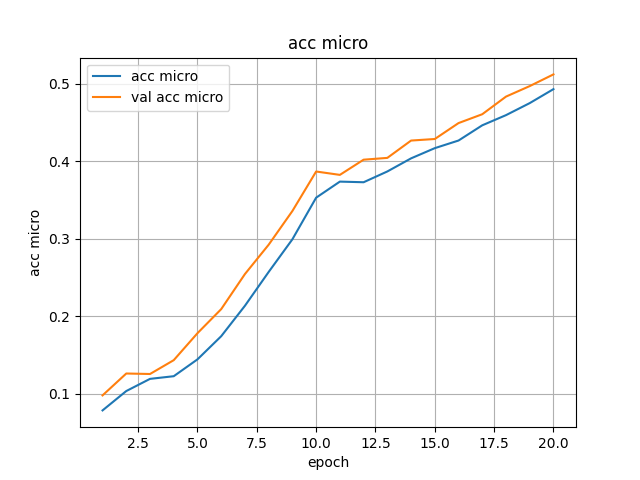
\includegraphics[width=\linewidth]{../logs/supertag/acc micro.png}
    \end{subfigure}
    \begin{subfigure}{0.32\textwidth}
        \centering
        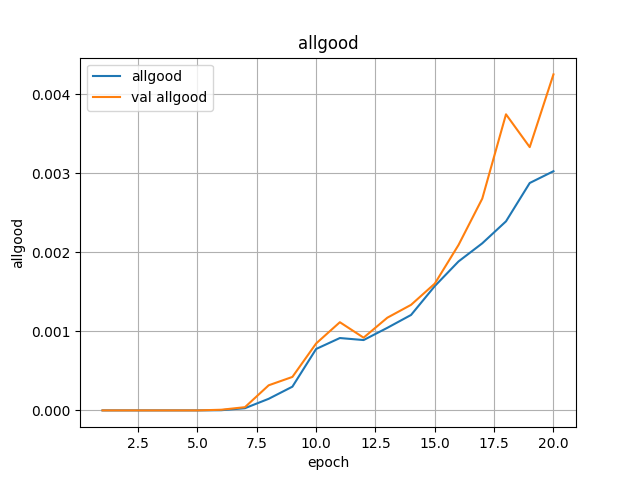
\includegraphics[width=\linewidth]{../logs/supertag/allgood.png}
    \end{subfigure}
    \caption{Valeurs de la loss et des métriques d'entraînement et de validation en fonction des epochs 
            pour le modèle \textit{SUPERTAG}.}
    \label{fig: results supertag}
\end{figure}

L'apprentissage est satisfaisant, car les courbes d'entraînement et de validation suivent la même allure d'après les 
Figures~\ref{fig: model supertag}. 
On peut expliquer la meilleure performance
de la validation par rapport à l'entraînement par l'utilisation du dropout dans l'apprentissage. Cette méthode est présente lors
de l'entraînement, ce qui va naturellement baisser ses performances. 
Néanmoins, il y a un risque de overfitting lorsque l'on considère le modèle selon l'accuracy allgood. 

\begin{figure}[H]
    \centering
    \begin{subfigure}{0.32\textwidth}
        \centering
        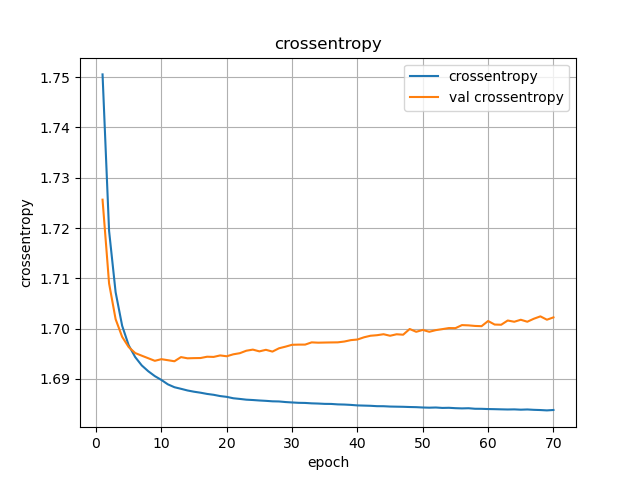
\includegraphics[width=\linewidth]{../logs/separate/crossentropy.png}
    \end{subfigure}
    \begin{subfigure}{0.32\textwidth}
        \centering
        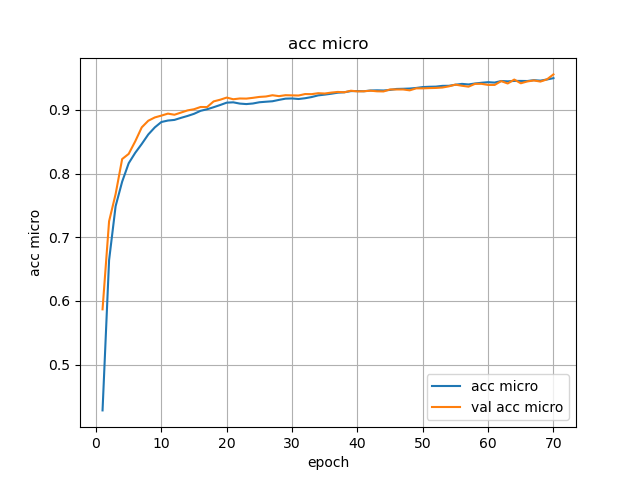
\includegraphics[width=\linewidth]{../logs/separate/acc micro.png}
    \end{subfigure}
    \begin{subfigure}{0.32\textwidth}
        \centering
        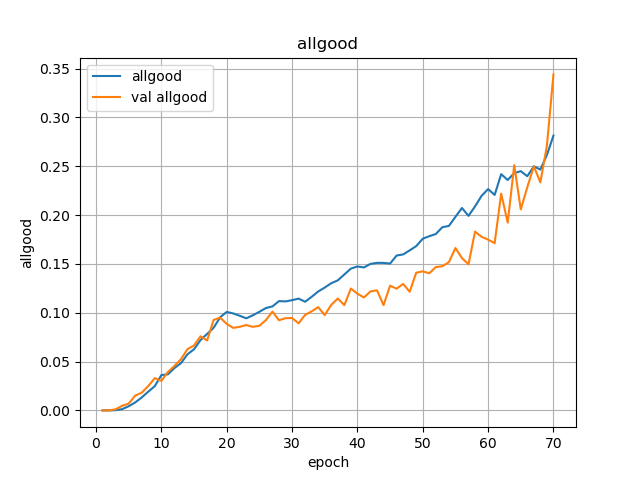
\includegraphics[width=\linewidth]{../logs/separate/allgood.png}
    \end{subfigure}
    \caption{Valeurs de la loss et des métriques d'entraînement et de validation en fonction des epochs 
            pour le modèle \textit{SEPARATE}.}
    \label{fig: results separate}
\end{figure}

Le modèle \textit{SEPARATE} témoigne d'un apprentissage satisfaisant, où par rapport au modèle précédent, le risque d'overfitting 
semble plus faible selon l'accuracy et allgood, avec néanmoins de l'instabilité qui subsiste, d'après les 
Figures~\ref{fig: results separate}.

\begin{figure}[H]
    \centering
    \begin{subfigure}{0.32\textwidth}
        \centering
        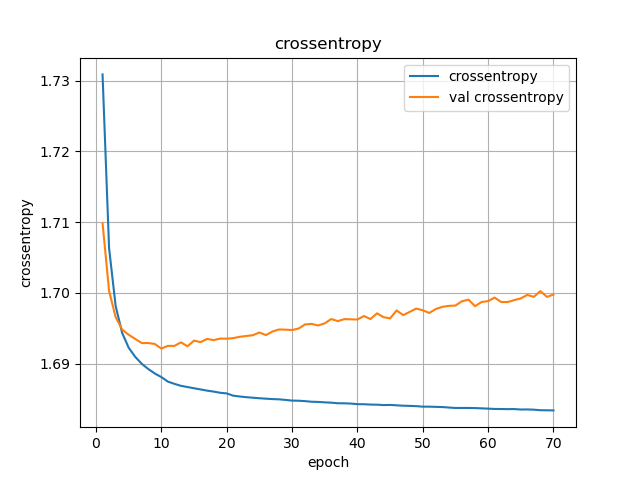
\includegraphics[width=\linewidth]{../logs/fusion/crossentropy.png}
    \end{subfigure}
    \begin{subfigure}{0.32\textwidth}
        \centering
        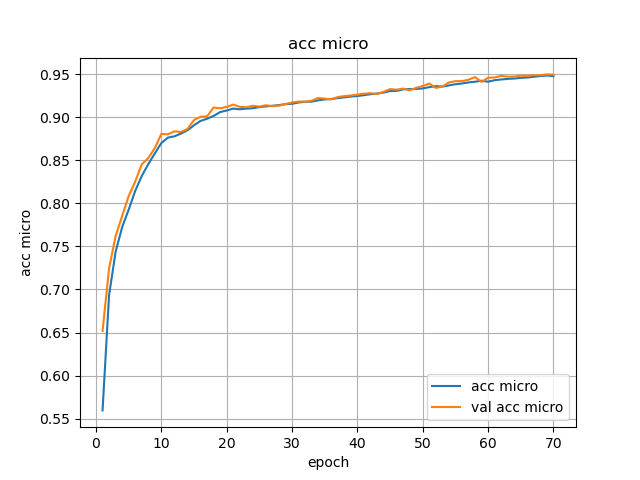
\includegraphics[width=\linewidth]{../logs/fusion/acc micro.png}
    \end{subfigure}
    \begin{subfigure}{0.32\textwidth}
        \centering
        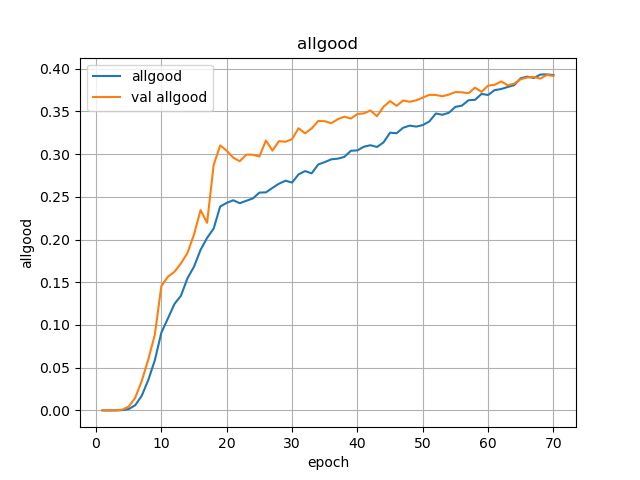
\includegraphics[width=\linewidth]{../logs/fusion/allgood.png}
    \end{subfigure}
    \caption{Valeurs de la loss et des métriques d'entraînement et de validation en fonction des epochs 
            pour le modèle \textit{FUSION}.}
    \label{fig: results fusion}
\end{figure}

Le modèle \textit{FUSION} témoigne d'un apprentissage satisfaisant et relativement meilleur que celui des modèles précédents, à 
travers les Figures~\ref{fig: model fusion}.


\begin{table}[H]
    \centering
    \begin{tabular}{|c|c|c|c|}
        \hline
         Nom du modèle & crossentropy & accuracy micro & all good\\
         \hline
         \textit{BASELINE}& - & 0.980 & 0.791 \\
         \hline
         \textit{SUPERTAG}& 1.700 & 0.436 & 0.002\\
         \hline
         \textit{SEPARATE}& 1.70 & 0.893 & 0.046\\
         \hline
         \textit{FUSION}& 1.698 & 0.884 & 0.154 \\
         \hline
    \end{tabular}
    \caption{Résultats de test sur la prédiction des \textit{morphy}}
    \label{tab: test morphy}
\end{table}

Les résultats du Table~\ref{tab: test morphy} mettent en comparaison les résultats de performances entre les modèles.
Le modèle baseline indique une performance d'accuracy de 98\% et donne les autres.
Entre les trois autres modèles, c'est le modèle \textit{SEPARATE} qui performe le mieux en termes d’accuracy micro, cependant,
c'est le modèle \textit{FUSION} qui performe le mieux en termes d’accuracy allgood. 

Néanmoins, ces modèles ne permettent pas de dépasser les performances de la baseline, alors que les modèles implémentés ont une
significative complexité plus importante que celle de la baseline.
Ce qui se peut s'expliquer principalement parce que les \textit{morphy} des mots ne changent presque jamais, cela avantage 
énormément la baseline.

\section{Inférences}

Nous avons ensuite testé nos différents modèles en leurs faisant prédire les \textit{morphy} sur une phrase. Nous avons fait
l'inférence sur la phrase : \textit{Les bananes sont jaunes et mûrs.}. Comme cette phrase n'a que 7 mots (6 mots et un point),
on rajoute 3 caractères de padding <PAD>. Les Tables~\ref{tab: bananes} et \ref{tab: lastpad} représentent respectivement les
\textit{morphy} prédit par les modèles du mot \textit{bananes} et du dernier <PAD>.
\begin{table}[H]
    \centering
    \begin{tabular}{|c|c|}
        \hline
        \textbf{modèle} & \textbf{inférences} \\
        \hline
        \textit{BASELINE} & Gender=Fem$\mid$Number=Plur \\
        \hline
        \textit{SUPERTAG} & NumForm=Roman$\mid$Abbr=Yes$\mid$Morph=VInf\\
        \hline
        \textit{SEPARATE} & Gender=Neut$\mid$Number=Plur$\mid$VerbForm=Ger\\
            & Degree=Pos$\mid$Abbr=Yes\\
        \hline
        \textit{FUSION} & Gender=Fem,Masc$\mid$Number=Plur$\mid$PronType=Tot\\
            & NumType=Mult$\mid$Case=Nom$\mid$NumForm=Combi\\
        \hline
    \end{tabular}
    \caption{Inférences du mot \textit{bananes}}
    \label{tab: bananes}
\end{table}

\begin{table}[H]
    \centering
    \begin{tabular}{|c|c|}
        \hline
        \textbf{modèle} & \textbf{inférences} \\
        \hline
        \textit{BASELINE} & <PAD>=Yes \\
        \hline
        \textit{SUPERTAG} & PronType=Emp$\mid$Style=Coll\\
        \hline
        \textit{SEPARATE} & <PAD>=Yes$\mid$PronType=Int,Rel$\mid$Case=Nom\\
            & Degree=Sup$\mid$NumForm=Combi\\
        \hline
        \textit{FUSION} & <PAD>=Yes$\mid$Gender=Neut$\mid$PronType=Int,Rel\\
            & NumType=Mult$\mid$Degree=Sup$\mid$Style=Slng\\
            & NumForm=Combi\\
        \hline
    \end{tabular}
    \caption{Inférences du dernier <PAD>.}
    \label{tab: lastpad}
\end{table} 

Le modèle \textit{SEPARATE}, pour le dernier <PAD>, prédit bien du <PAD> mais également d'autres 
labels qui n'ont rien à voir et qui sont incorrects. Une raison peut-être que la séparation des couches présentes dans notre modèle 
implique que certaines couches denses ne communiquent plus entre elles à une certaine étape de notre modèle pour réaliser leur 
inférence.

D'autre part, le modèle \textit{FUSION} prédit un nombre superflu de labels de manière générale, plus que nécessaire. Le modèle 
combine non seulement cette architecture de séparation de couches denses pour différentes classes, mais également une fusion qui multiplie alors le nombre de labels inféré. 

Dans cette perspective d'inférence, le modèle \textit{SUPERTAG} semble relativement plus pertinent en fournissant un nombre 
relativement plus raisonnable, cependant, il reste non adapté étant donné que ces prédictions sont tout simplement incorrectes. 

L'inférence fait ressortir différentes problématiques des architectures adoptées pour nos modèles.

\section{Conclusion}

Nous avons exploré deux tâches principales : l'étiquetage des parties du discours (\textit{pos}) et la prédiction des traits
morphologiques (\textit{morphy}). 

Le modèle \textit{GET\_POS} a démontré des performances impressionnantes dans la prédiction des parties du discours, avec une
accuracy micro de 94.4\% et une accuracy macro de 81.6\% sur le jeu de test. Ces résultats témoignent de la capacité du modèle
à apprendre efficacement la structure grammaticale des phrases en français.

Pour la tâche de prédiction des traits morphologiques, trois architectures de modèles ont été développées : \textit{SUPERTAG},
\textit{SEPARATE}, et \textit{FUSION}. Chacun de ces modèles a présenté des performances variées. Le modèle \textit{SEPARATE} a
obtenu une accuracy micro de 89.3\% et une métrique \textit{all good} de 4.6\%, montrant sa capacité à prédire les traits
morphologiques pour chaque classe. Cependant, le modèle \textit{FUSION} a montré une instabilité lors de l'entraînement, ce
qui peut nécessiter des ajustements pour améliorer ses performances.

Néanmoins, ces performances sont à prendre avec du recul et à nuancer, car nos résultats d'inférences sont assez décevants. Cela est 
sûrement dû à des problématiques intrinsèques aux architectures adoptées dans nos modèles, ce qui mérite une investigation plus 
poussée et des perspectives à étudier. 

Les résultats obtenus ouvrent des perspectives intéressantes pour l'amélioration des modèles de langage, en particulier dans le
contexte du Français. Des ajustements futurs pourraient inclure des stratégies plus sophistiquées pour la gestion des mots
inconnus et des expériences avec d'autres architectures de modèles.

Ce projet a donc permis d'explorer différentes facettes de la modélisation du langage, de la prédiction des parties du discours à
la prédiction des traits morphologiques. Les résultats obtenus constituent une base solide pour des développements futurs dans le
domaine de la compréhension automatique du langage naturel en français.


\section{Annexes}
\label{sec: Annexes}

\begin{figure}[H]
    \centering
    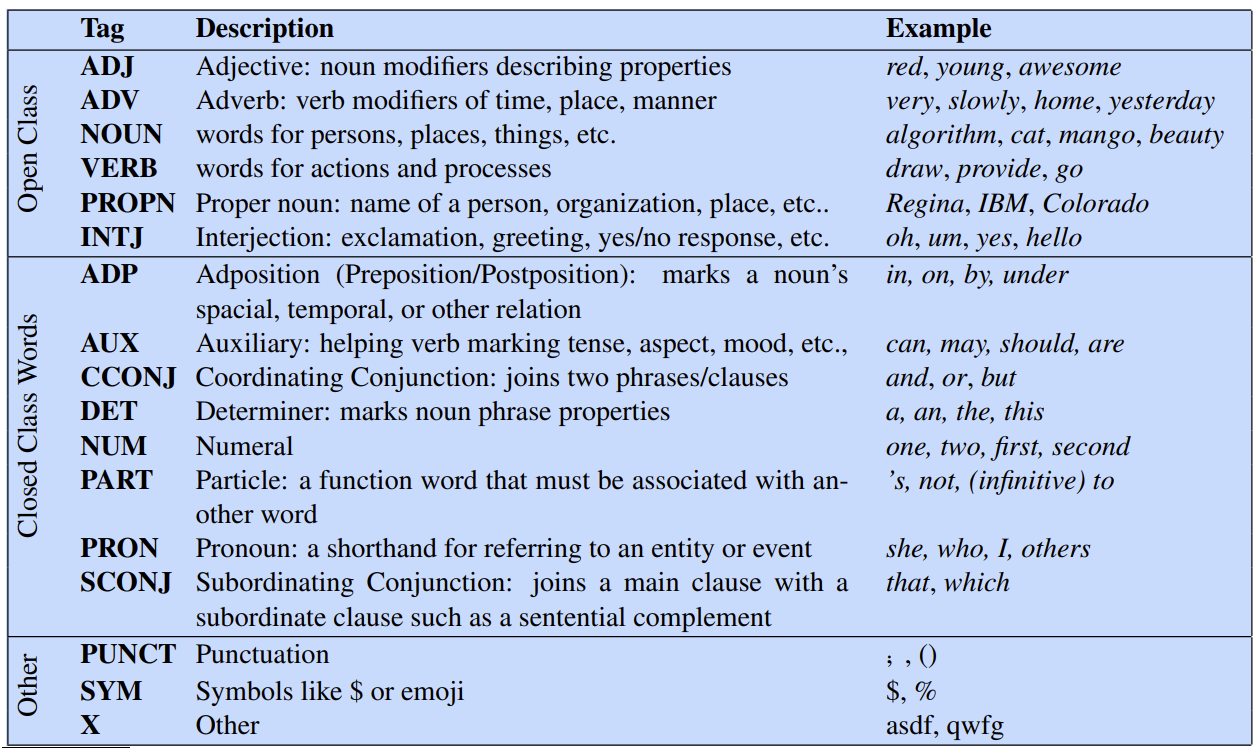
\includegraphics[width=0.9\textwidth]{all_pos.png}
    \caption{Liste des labels \textit{pos}. Image tirée de~\cite{pos}}
    \label{fig: all pos}
\end{figure}   

\begin{figure}[H]
    \centering
    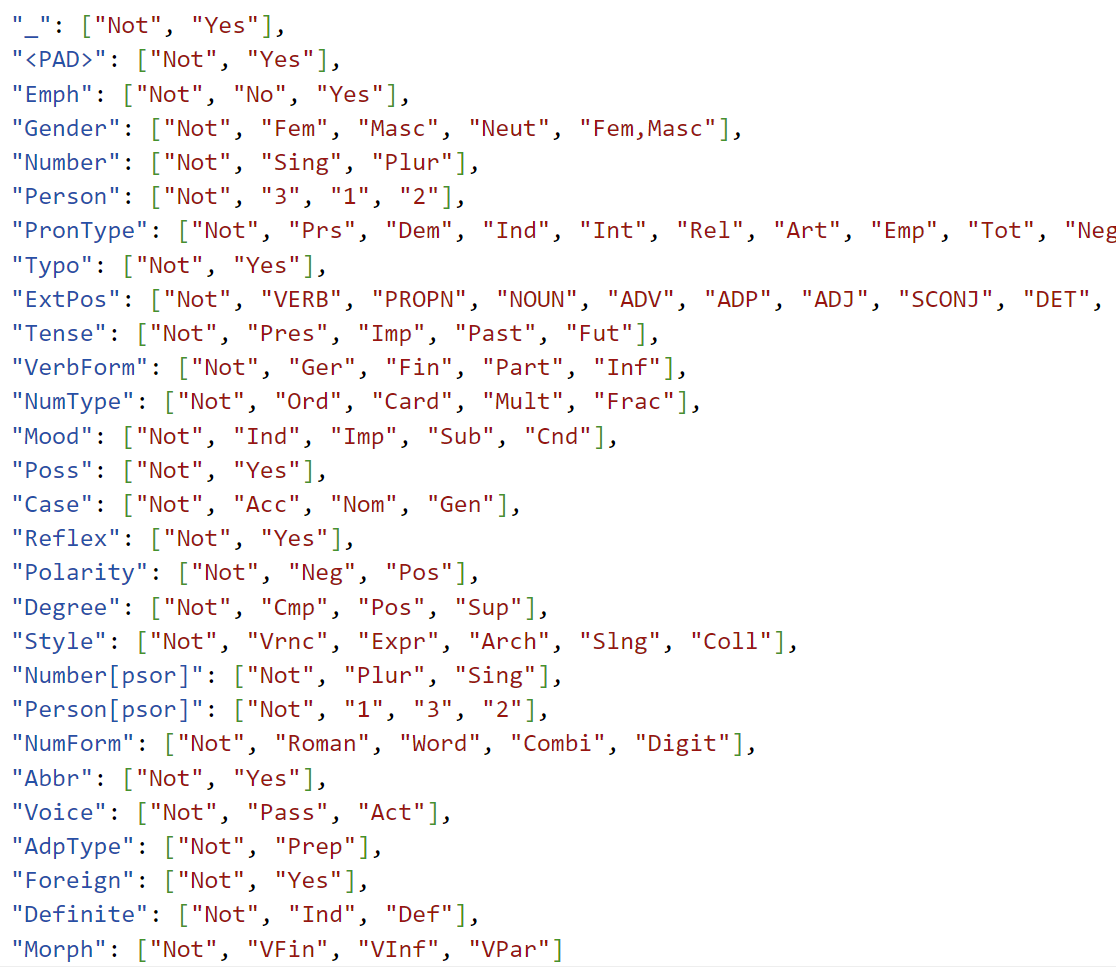
\includegraphics[width=0.9\textwidth]{all_morphy.png}
    \caption{Liste des \textit{morphy}}
    \label{fig: all morphy}
\end{figure}  

\bigskip
\printbibliography


\end{document}